%% Copernicus Publications Manuscript Preparation Template for LaTeX Submissions
%% ---------------------------------
%% This template should be used for copernicus.cls
%% The class file and some style files are bundled in the Copernicus Latex Package, which can be downloaded from the different journal webpages.
%% For further assistance please contact Copernicus Publications at: production@copernicus.org
%% https://publications.copernicus.org/for_authors/manuscript_preparation.html


%% Please use the following documentclass and journal abbreviations for discussion papers and final revised papers.

%% 2-column papers and discussion papers
\documentclass[gmd, manuscript]{copernicus}

%% \usepackage commands included in the copernicus.cls:
%\usepackage[german, english]{babel}
%\usepackage{tabularx}
%\usepackage{cancel}
%\usepackage{multirow}
%\usepackage{supertabular}
%\usepackage{algorithmic}
%\usepackage{algorithm}
%\usepackage{amsthm}
%\usepackage{float}
%\usepackage{subfig}
%\usepackage{rotating}


\begin{document}

\title{The analysis of large-volume multi-institute climate model output at a Central Analysis Facility (PRIMAVERA Data Management Tool V2.10)}


% \Author[affil]{given_name}{surname}

\Author[1]{Jon}{Seddon}
\Author[2]{Ag}{Stephens}
\Author[1]{Matthew S.}{Mizielinski}
\Author[3]{Pier Luigi}{Vidale}
\Author[1]{Malcolm J.}{Roberts}

\affil[1]{Met Office Hadley Centre, FitzRoy Road, Exeter, EX1 3PB, UK}
\affil[2]{Centre for Environmental Data Analysis, RAL Space, STFC Rutherford Appleton Laboratory, Harwell, Oxford, Didcot, OX11 0QX, UK}
\affil[3]{NCAS-Climate, Department of Meteorology, University of Reading, Reading, RG6 6AH, UK}

%% The [] brackets identify the author with the corresponding affiliation. 1, 2, 3, etc. should be inserted.



\runningtitle{TEXT}

\runningauthor{TEXT}

\correspondence{Jon Seddon (jon.seddon@metoffice.gov.uk)}



\received{}
\pubdiscuss{} %% only important for two-stage journals
\revised{}
\accepted{}
\published{}

%% These dates will be inserted by Copernicus Publications during the typesetting process.


\firstpage{1}

\maketitle



\begin{abstract}
The PRIMAVERA project aimed to develop a new generation of advanced and well-evaluated high-resolution global climate models. As part of PRIMAVERA, seven different climate models were run in both standard and higher resolution configurations, with common initial conditions and forcings to form a multi-model ensemble. The ensemble simulations were run on high performance computers across Europe and generated approximately 1.6~pebibytes of output. To allow the data from all models to be analysed at this scale, PRIMAVERA scientists were encouraged to bring their analysis to the data. All data was transferred to a Central Analysis Facility (CAF), in this case the JASMIN super-data-cluster, where it was catalogued and details made available to users using the PRIMAVERA Data Management Tool's (DMT's) web interface. Users from across the project were able to query the available data using the DMT and then access it at the CAF. Here we describe how the PRIMAVERA project used the CAF's facilities to enable users to analyse this multi-model data set. We believe that PRIMAVERA's experience using a CAF demonstrates how similar, multi institute, big-data projects can efficiently share, organise and analyse large volumes of data.
\end{abstract}


\copyrightstatement{The works published in this journal are distributed under the Creative Commons Attribution 4.0 License. This licence does not affect the Crown copyright work, which is re-usable under the Open Government Licence (OGL). The Creative Commons Attribution 4.0 License and the OGL are interoperable and do not conflict with, reduce or limit each other.

\noindent\textcopyright~Crown copyright 2023}


\introduction  %% \introduction[modified heading if necessary]

The PRIMAVERA project aimed to develop a new generation of advanced and well-evaluated high-resolution global climate models. Two ``streams'' of simulations were performed within PRIMAVERA, each consisting of seven different climate models (AWI-CM-1-1, CMCC-CM2, CNRM-CM6-1, EC-Earth3P, ECMWF-IFS, HadGEM3-GC31 and MPI-ESM1-2) that were run at their standard nominal resolution~\citep{GloablAttr} (typically  250~km in the atmosphere and 100~km in the ocean) and at a higher resolution (25~km atmosphere and 8-25~km ocean). All models were run with common initial conditions and forcings according to the HighResMIP protocol~\citep{Haarsma2016}. The simulations were run on high performance computers (HPCs) across Europe and the more than 100 scientists who analysed the data were based at 20 different institutes across Europe with assistance from other global scientists. Perhaps the most challenging aspect of working with global, high-resolution simulations is the volume of data produced. High-resolution simulations have been shown to better represent many different aspects of the climate, such as tropical cyclones~\citep{Roberts2020} and atmospheric blocking~\citep{Schiemann2019}. The PRIMAVERA simulations generated a total of 1.6~pebibytes (PiB) of data\footnote{Data volumes and rates in this paper use binary prefixes and so 1~PiB is $1024^5$~bytes~\citep{IEEE1541}.}.

A Data Management Plan (DMP) was developed to allow this data to be stored, analysed and archived at a Central Analysis Facility (CAF), which in PRIMAVERA's case was the JASMIN super-data-cluster. The Data Management Tool (DMT) software was written to implement the DMP and provides the ability to catalogue and then search the project's data. The DMT tracked and controlled the movement of individual files as they are moved between tape and disk, and allowed the data to be published to the global community for sharing at the end of the project.

If a CAF had not been available for PRIMAVERA to use then it would have been necessary for each modelling centre to make their own data available, typically on an Earth System Grid Federation (ESGF) node~\citep{ESGFCinquini}\citep{gmd-14-629-2021} or local File Transfer Protocol (FTP) server. Anyone wanting to analyse data would have needed to identify which variables were available and then download them from each modelling centre to their home institute. There would have been multiple copies of common datasets and each institute would have required significant volumes of storage, transfer bandwidth and compute resources.

In this paper we introduce the CAF and the PRIMAVERA project. We then describe the DMP and DMT and explain how they allowed the project's data to be managed. Finally, we provide a summary of how the data was transferred to the CAF and describe some of the hardware and software opportunities that may be suitable for managing similar projects in the future.

\section{The Central Analysis Facility}

The CAF used in the PRIMAVERA project is JASMIN, a super-data-cluster that was installed in 2012 \citep{lawrence2013storing}. It is funded by the Natural Environment Research Council (NERC) and the United Kingdom (UK) Space Agency, and operated by the Science and Technology Facilities Council (STFC). It is located at the STFC Rutherford Appleton Lab (RAL), Harwell, UK. JASMIN's Phase 4 update in September 2018 added 38.5~PiB of new storage co-located with the existing 4000 cores of compute. The storage and compute are tied together with a low latency network. RAL has a fast connection to Janet, the UK's academic network, which in turn is connected to the G\'{E}ANT European network, allowing the fast transfer of data from the HPCs used to run the PRIMAVERA simulations to JASMIN. In addition, JASMIN is connected to an on-site tape library for the offline storage of data. Similar CAFs exist at Centro Euro-Mediterraneo sui Cambiamenti Climatici (CMCC)~\citep{CMCC}, Deutsches Klimarechenzentrum (DKRZ, German Climate Computing Centre)~\citep{dkrz} and at Lawrence Berkeley National Laboratory on the Cori supercomputer~\citep{cori}.

The compute at JASMIN is split into interactive data analysis servers, the LOTUS batch processing system and some additional private cloud servers. Part of the storage is dedicated for the Centre for Environmental Data Analysis (CEDA) archive, which contains over 13~PiB of atmospheric and earth observation data, and is connected to the UK's ESGF node. The co-location of the storage, datasets in the archive and compute makes JASMIN a powerful facility to analyse climate simulations with.

All compute hosts at JASMIN run the Linux operating system and have a suite of modern software tools and programming languages installed for the analysis and manipulation of common Earth science data formats. The storage for individual projects is split into allocations called group workspaces (GWS) each of which is up to 100~tebibytes (TiB).

\section{PRIMAVERA}

The Horizon 2020 funded PRIMAVERA project was made up of eleven work packages (WPs)~\citep{GrantAgree} covering a range of scientific, technical, management, communication and user engagement topics. The Stream 1 and 2 simulations described here were run and managed by two of the work packages. Several of the other WPs analysed these simulations and compared them with existing simulations, observations and reanalyses. The remaining WPs carried out model development work or ran small simulations that did not need to be shared with other WPs. These WPs only required a small volume of storage on one of the GWS.

The Stream 1 and 2 simulations follow the HighResMIP protocol and have been submitted to the 6th phase of the Coupled Model Intercomparison Project (CMIP6) \citep{Eyring2016}. The Stream 1 simulations consist of a single ensemble member from each model at a standard and a high resolution for six different experiments. The follow-on Stream 2 simulations contain additional ensemble members for the experiments performed in Stream 1, but with a reduced data output to minimise the volume of data generated plus some additional simulations to exploit the new physics modules (for example~\citep{Nurser2020}) that have been developed in PRIMAVERA.

Due to the scientific complexity, data volumes and geographical distribution of the project participants, it was recognized that developing and implementing a data management plan would require a significant amount of time and effort. Sufficient resource was included in the project proposal to allow for this development work.


\section{Data Management Plan}

\begin{figure*}[t]
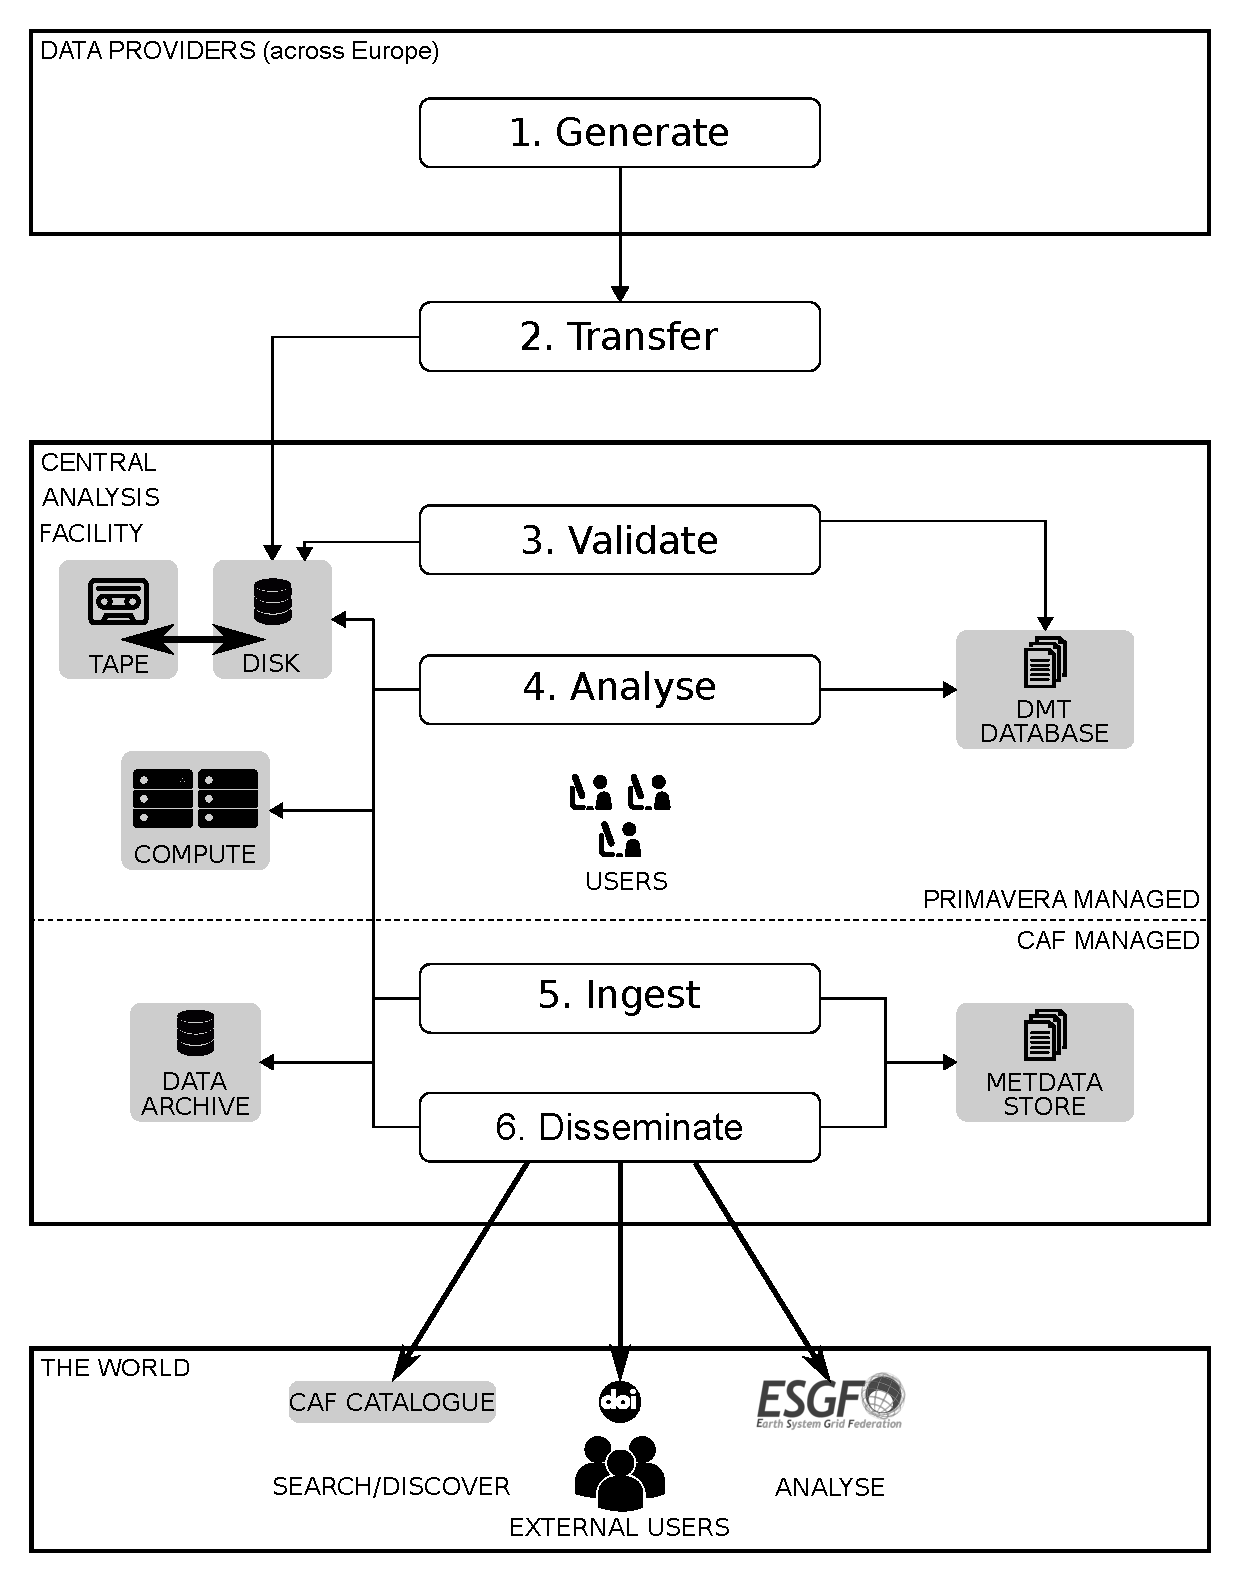
\includegraphics[width=12cm]{fig01.pdf}
\caption{The workflow developed for PRIMAVERA in the Data Management Plan.}
\label{dmp_workflow}
\end{figure*}

The PRIMAVERA Data Management Plan~\citep{Mizielinski2016} can be summarised as ``taking the analysis to the data''. Figure~\ref{dmp_workflow} shows the workflow developed in the DMP. All data files from the PRIMAVERA simulations were uploaded to the CAF and made accessible to project members, who were able to undertake their analysis of them. It has been common practise in many climate science projects to download the required data and perform analyses locally at users' home institutes. Early analysis of the data requirements of the PRIMAVERA project, along with experience from prior projects, indicated that the downloading and local analysis of data would lead to significant technical challenges for each institute. As such, central analysis facilities such as JASMIN that provide data storage and compute are key to the exploitation of big data projects such as PRIMAVERA and CMIP6.

The first step in the DMP workflow is the generation of data by the modelling centres; simulations are run on a variety of HPCs across Europe and each model typically has its own proprietary output file format. As PRIMAVERA made up the majority of the European contribution to HighResMIP it was necessary to conform to the  CMIP6 data standards~\citep{gmd-11-3659-2018}. These standards require data to be provided in CMOR3 (Climate Model Output Rewriter)~\citep{Nadeau2019} compliant netCDF files following the CMIP6 conventions. Where data had been generated in a proprietary format it was post-processed to comply with these standards.

The second step in the workflow is the transfer of the data from the HPCs or post-processing systems to the CAF. A discussion on the transfer techniques used and the rates achieved is given in Sect.~\ref{transfer_rates}. The data is uploaded to the PRIMAVERA storage volume at the CAF.

The data sets provided are passed through a quality control process in step 3, which includes checking that the data and metadata standards have been complied with, and the extraction of metadata to store in the DMT's database~\citep{Seddon2020}. After completion of the validation process, files are archived to tape and removed from the GWS to create space for other uploads. After the upload and validation of the data, users analyse and work with it in Step 4. 

The final steps in the workflow (steps 5 and 6 in Fig.~\ref{dmp_workflow}) are managed by CEDA rather than the PRIMAVERA project as these relate to the use of shared facilities. Uploaded data is ingested into the CEDA archives~\citep{CEDAArchive} and is then available for dissemination to the global community using the CEDA Earth System Grid Federation node~\citep{CEDAESGF}. Steps 5 and 6 do not have to be run immediately after the data has been validated. A delay before dissemination to the global community allows the project's users to have a period of sole access to the data and the opportunity to generate the first publications from the simulations.


\subsection{CAF Resources}

After reviewing the DMP, PRIMAVERA was allocated 440~TiB of storage at the CAF split across five volumes. A virtual machine in the internal cloud was provided, which was given a domain name and HTTPS access allowed to it from the Internet, and the DMT software and database were installed on this server.

The 440~TiB of storage at the CAF that was allocated to the project was 2.4~\% of the almost 18~PiB of project storage allocated to all 242 group workspaces at JASMIN in March 2021~\citep{Townsend2021}. 100 PRIMAVERA users were 4.1~\% of the total number of the CAF's users at the same time. 

It was originally estimated that around 2.4~PiB of data would be generated by the project, and therefore only a subset of data could be held on disk at once. The remaining data would have to be held on tape and moved to the GWS as required. The DMP describes how the DMT would allow data to be efficiently and reliably moved between tape and GWS and its location tracked.

\subsection{Typical Analysis Workflow}

\begin{figure*}[ht]
	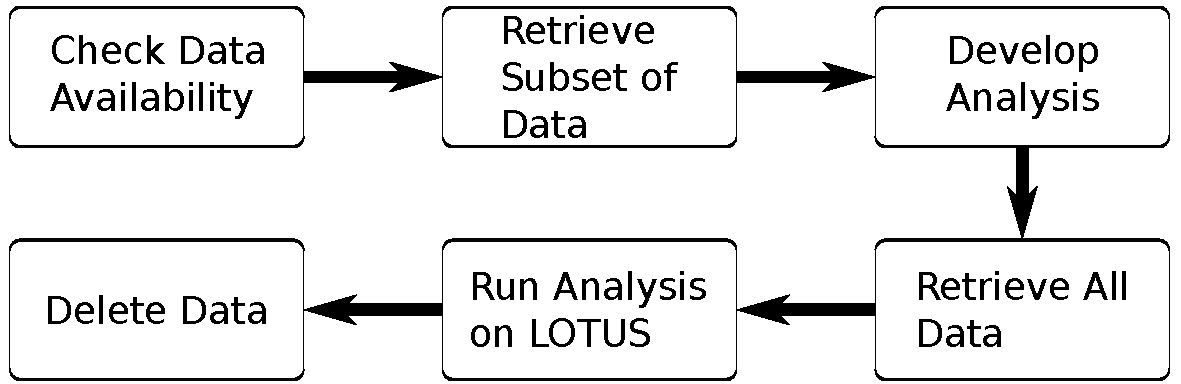
\includegraphics[width=8.3cm]{fig02.pdf}
	\caption{The workflow used by users working with the PRIMAVERA data at the CAF.}
	\label{analysis_workflow}
\end{figure*}

Figure~\ref{analysis_workflow} shows the workflow that users working with the PRIMAVERA data at the CAF were required to follow. Users began by using the DMT's web interface to identify what data had been uploaded. If the data they required was not available on disk then they used the DMT's web interface to request that a subset of their data was restored from tape to disk. The DMT sent them an email when this requested sample dataset was available on disk and they could then work on the CAF's interactive servers to develop and test their analysis code. After testing and validating their analysis code, they could then use the DMT to request that all of the data they required was restored from tape to disk. Once the full dataset was available on the GWS then the analysis was run on the LOTUS batch processing cluster. When their analysis was complete, users then marked the data as finished in the DMT's web interface and the DMT would then delete the data from disk to create space for other data. This workflow allowed for the efficient use of disk space; PRIMAVERA generated over 1.6~PiB of data but the upload of data, analysis and some storage of additional observations and reanalyses was able to fit into 440~TiB of allocated disk space.

\section{Data Management Tool}

The DMT was developed to track and control the flow of PRIMAVERA data around the CAF and to allow users to query the available data and its location. It was built upon a PostgreSQL database and custom software written in the Python programming language, using the Django web framework~\citep{Django}. The database was installed on a dedicated server, along with web server software and the DMT application, and was accessible to users across all hosts at the CAF. Access to the database from the compute cluster allowed the batch submission of validation processes to the  compute cluster allowing significant parallelisation of the work.

\begin{figure*}[ht]
	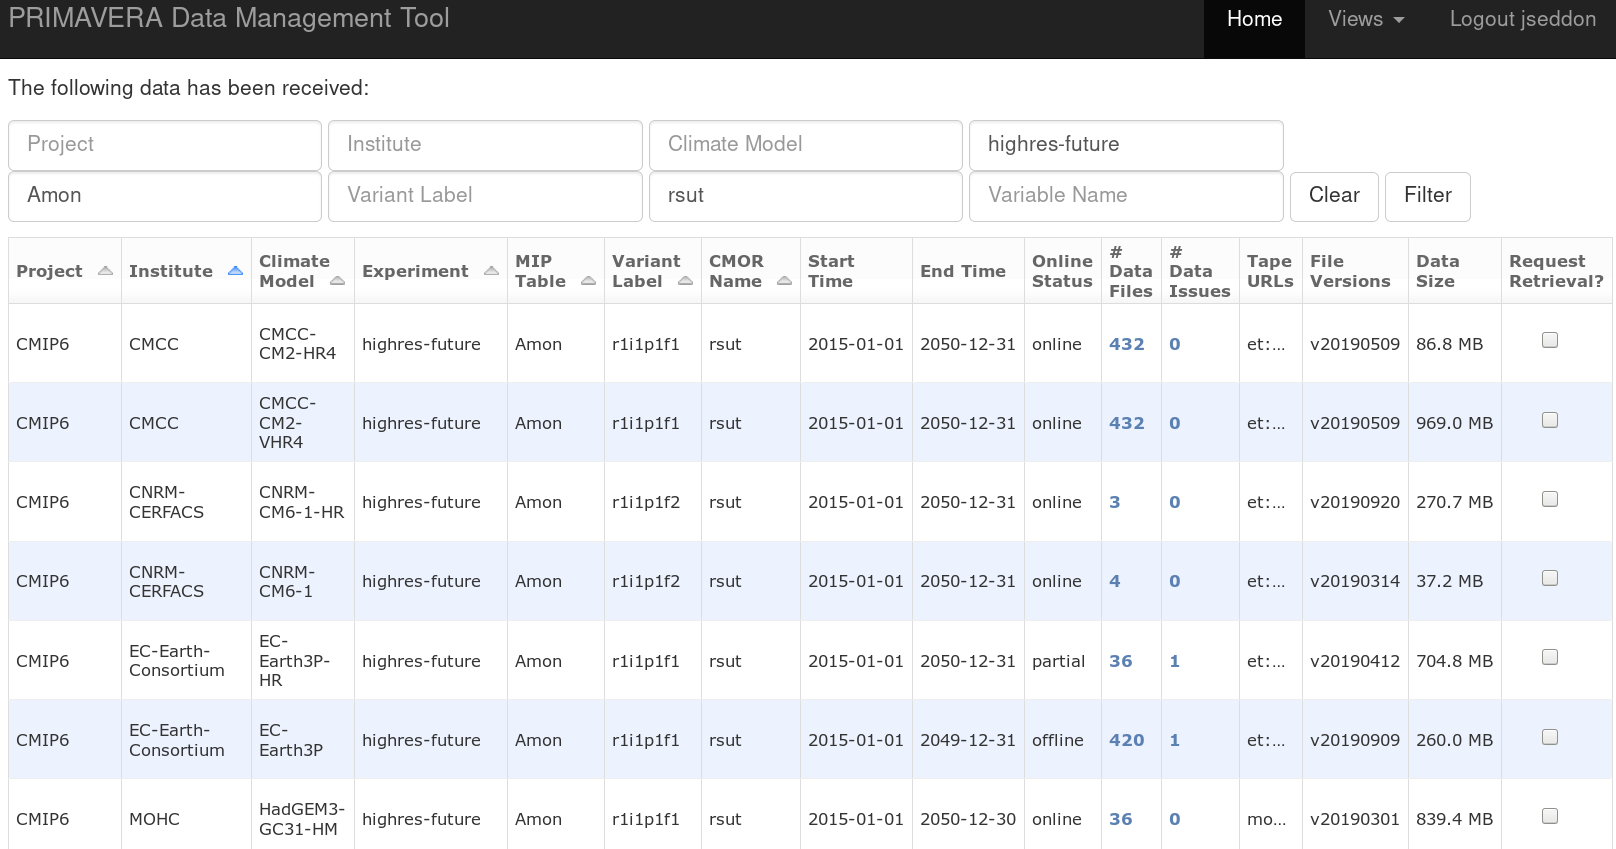
\includegraphics[width=12cm]{fig03.png}
	\caption{A screenshot from the DMT's web interface showing the data available for one variable from the coupled future experiment.}
	\label{dmt_query}
\end{figure*}

A typical screenshot from a user querying the DMT's web interface is shown in Fig.~\ref{dmt_query}. In this example the variable ``rsut'', the top of atmosphere outgoing shortwave radiation, from the ``highres-future'' coupled future experiment is being queried. A value of ``offline'' in the ``Online Status'' column shows that the files for this simulation are currently only available on tape, a value of ``partial'' shows that some files are on disk, but others are only available on tape and ``online'' shows that all files are available on disk. The ``Request Retrieval?'' column allows users to indicate that they want to work with this variable. If the variable's files need to be restored from tape to disk then they are queued for retrieval and the user is emailed when the data becomes available. The DMT contains a similar page to allow users to view the data that they have requested and to mark it as used, so that it can be deleted from disk to release storage.

The DMT software~\citep{Seddon2019} is distributed under an open source license. Development of the DMT began in April 2016 and the first data was made available via the DMT in May 2017, requiring the full time work of one developer. Development work has continued as required since then to improve the flow of data through the system and to facilitate the publication of data to the ESGF. 

\subsection{DMT Internal Structure}

\begin{figure*}[ht]
	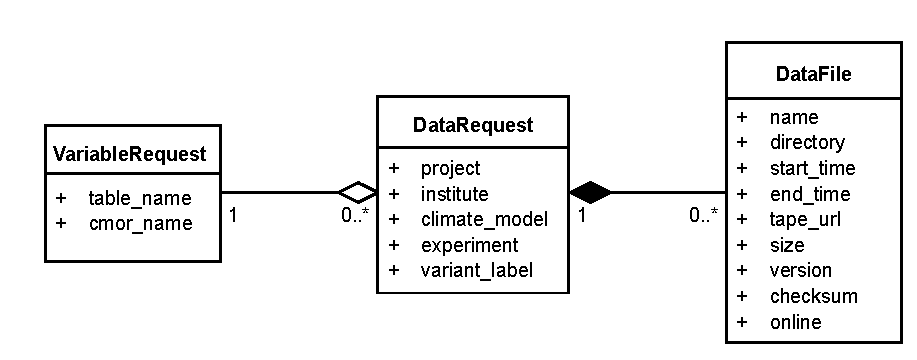
\includegraphics[width=12cm]{fig04.pdf}
	\caption{A simplified UML class diagram showing how data requests and data files are implemented as Django models in the DMT.}
	\label{dmt_struture}
\end{figure*}

Figure~\ref{dmt_struture} shows a simplified UML class diagram showing how data is represented as Django models, implemented as Python classes in the DMT. Internally, the DMT's primary data object is a DataRequest. A DataRequest object consists of a VariableRequest object along with details of the institute, climate model, experiment and variant label. The VariableRequest object specifies a CMIP6 variable and MIP table along with additional metadata. VariableRequest objects are created programmatically from the CMIP6 HighResMIP data request~\citep{Juckes2020}. During the development of the data management plan, a shared spreadsheet was created from the HighResMIP data request and each institute edited the spreadsheet to indicate the variables that they would generate. The DataRequest objects were created programmatically from this spreadsheet. A facility to allow institutes to update the data requests that they would provide during the project was developed to allow for changes to institutes' plans.

A DataFile object was created for each file uploaded to the CAF during the validation process and a checksum was calculated for each file submitted to the DMT. The checksums were used throughout the workflow as files were moved from tape to disk to ensure their integrity. Each DataFile is related to a DataRequest and all views in the DMT's web interface are generated from these DataRequest objects. All objects are mapped to database tables using Django's object-relational mapper. 

The DMT worked well, although some effort was required to maintain the set of expected data requests. Programmatically creating data requests  when each file is validated and added to the DMT would have been more efficient.

\section{Data Transfer}
\label{transfer_rates}

\begin{table}[ht]
	\caption{The rates achieved while transferring data from the data providers to the CAF.}
	\begin{tabular}{lll}
		\tophline
		Transfer from & Rate achieved & Protocol used \\
		\middlehline
		Toulouse, France & 13~MiB~s$^{-1}$ & 4 BBCP jobs in parallel, with 4 streams each \\
		Hamburg, Germany & 20 to 55~MiB~s$^{-1}$ & globus-url-copy \\
		Lecce, Italy & 34~MiB~s$^{-1}$ average, 69~MiB~s$^{-1}$ peak & gridftp, with 4 concurrent FTP connections 8 process in parallel \\
		Bologna (Cineca), Italy & 200 to 300~MiB~s$^{-1}$ & 5 parallel \texttt{rsync -av -e "ssh -c arcfour"} \\
		Barcelona, Spain & 13~MiB~s$^{-1}$ & rsync \\
		Exeter, UK & 30~MiB~s$^{-1}$ & 5 groups of 3 FTP connections over dedicated link \\
		Reading, UK & 85~MiB~s$^{-1}$ & 4 parallel \texttt{rsync -rvz --rsh="ssh -c arcfour"} \\
		\bottomhline
	\end{tabular}
	\belowtable{} % Table Footnotes
	\label{rates_achieved}
\end{table}


Table~\ref{rates_achieved} shows the sustained rates achieved when transferring data from the data providers to the CAF in mebibytes per second (MiB~s$^{-1}$). JASMIN contains several servers in a data transfer zone, whose connection to the Internet and to the rest of the CAF has been designed for maximum data throughput. At the start of the project it had been assumed that parallel transfer protocols such as BBCP~\citep{bbcp} or GridFTP~\citep{Foster}\citep{Globus} would provide the best transfer rates and data providers were encouraged to use these. In reality, most data providers used the techniques that they were most familiar with as long as they gave sufficiently fast transfer rates. The rates achieved depend on many factors including the file systems, the load on the servers and the network between the servers. The fastest transfer rate from a site was over 200~MiB~s$^{-1}$, equivalent to 16.5 TiB per day. Typical rates were 30~MiB~s$^{-1}$ (2.5 TiB per day). These rates were sufficient to complete the project on time. It is hoped that with further optimisation work a sustained minimum transfer rate of 5.0~TiB per day could be achieved.

The collection of all of PRIMAVERA's data at the CAF was only possible because of the magnitude of the transfer rates that were achieved. If data transfer rates between the HPC centres and the CAF had been insufficient then the scientific analysis performed by PRIMAVERA would have been significantly impacted.

\section{Data Access and Analysis}

Because the DMT was used to restore data from tape to disk it is possible to analyse the fraction of data produced by the project that was analysed. As of 20th July 2020, 31,048 data requests had been uploaded to JASMIN containing 1.5~PiB of data. 6,070 unique data requests had been restored from tape to disk at least once, which is 20~\% of the data requests by number. However, these unique restored data requests contained 426~TiB of data, which is 27~\% of the volume of data that had been uploaded~\citep{Seddon2020b}. One reason that more data by volume than by number of data requests was requested could be because users were analysing the larger volume variables, which tend to be variables with a higher temporal frequency.

All of the data from the PRIMAVERA simulations was added to the CEDA archives and published to the ESGF. Because of the need to restore the data from tape, publication took over one year to complete.

In PRIMAVERA, users accessed the data using a variety of tools such as CDO~\citep{schulzweida_uwe_2022_7112925}, Python, Iris~\citep{Iris} and ESMValTool~\citep{Righi2020}. PRIMAVERA provided some resource for the development of ESMValTool, therefore much scientific analysis was completed before ESMValTool was available. ESMValTool may allow for the more efficient analysis of multi-model datasets in future projects.

\section{User Feedback}

\begin{table}[ht]
	\caption{Number of responses for each score from the users of the PRIMAVERA facilities at the CAF with 1 being very difficult and 7 being very easy.}
	\begin{tabular}{|c|c|p{15mm}|p{15mm}|p{15mm}|p{15mm}|p{15mm}|}
		\hline
		\multicolumn{2}{|c|}{} & Querying the data request to see which variables were scheduled to be produced. & Use of the DMT to discover and query the PRIMAVERA data available at JASMIN. & Retrieving data from tape to group workspace / disk. & Accessing the data on the JASMIN group workspaces. & Analysing the data at JASMIN?\\
		\hline
		\parbox[t]{2mm}{\multirow{7}{*}{\rotatebox[origin=c]{90}{Score}}} & 1 & 0 & 1 & 1 & 1 & 1\\
		& 2 & 1 & 1 & 0 & 1 & 0\\
		& 3 & 0 & 0 & 0 & 2 & 1\\
		& 4 & 0 & 0 & 1 & 0 & 2\\
		& 5 & 3 & 1 & 1 & 0 & 0\\
		& 6 & 7 & 11 & 10 & 7 & 8\\
		& 7 & 4 & 7 & 6 & 10 & 4\\
		\hline
		\multicolumn{2}{|c|}{\# Responses} & 15 & 21 & 19 & 21 & 16\\
		\hline
		\multicolumn{2}{|c|}{Mean} & 5.8 & 5.9 & 5.9 & 5.8 & 5.5\\
		\hline
	\end{tabular}
	\label{survey_responses}
\end{table}

A survey of all PRIMAVERA users of the CAF was conducted and responses were received from 24 users~\citep{Seddon2020c}. Users of the data were asked to rate five aspects of the process out of seven with 1 being very difficult and 7 being very easy and the results are shown in Table~\ref{survey_responses}. The response to all of the questions was midway between neutral and very easy to use. Four users did indicate that they had various levels of difficulty accessing the data and two users indicated some levels of difficulty analysing the data at the CAF; no additional feedback was provided explaining the difficulties that these users had encountered. The remaining 17 and 14 users respectively answered these two questions with neutral to very positive answers. These largely positive responses indicate that users had few problems performing their analyses at the CAF.

\section{Future Opportunities}

\subsection{Platforms}

\subsubsection{Central Analysis Facility}
Access to the CAF has been essential to the success of PRIMAVERA. JASMIN has a finite capacity and so may not be able to support all further projects that would benefit from having access to it. Central Analysis Facilities similar to JASMIN providing additional capacity would be incredibly useful for collaborative projects like PRIMAVERA as they would reduce the need for all institutes participating in a project to have their own large data storage and data analysis facilities. Such facilities also reduce the volume of data that needs to be transferred, which is important as climate simulations increase in resolution and complexity, and therefore increase in size.

Access to a CAF also allows scientists from some countries that do not currently have access to high-performance data analysis facilities locally to analyse large cutting-edge data sets. Some of these countries are on the front-line of climate change and access to a CAF would allow them to further contribute to climate science. For example, the CP4-Africa~\citep{Stratton2018} convection-permitting regional climate simulations over Africa are now available at JASMIN~\citep{Senior2019} and have been analysed at JASMIN by scientists working from Africa. Tools to access CAFs must be robust to the potentially slow and unreliable Internet connections that may be encountered in some countries. 

\subsubsection{Public Cloud}
Public cloud computing technologies could provide an alternative to a facility such as JASMIN. As users have been using local Unix based computers to analyse data for many years, the change from working locally to working remotely at JASMIN was therefore only a small change for users. The change was assisted by the CAF's comprehensive documentation~\citep{JASMINdocs} and the development of additional documentation and demonstration videos by the PRIMAVERA project. The CAF's mix of interactive servers and the batch processing cluster allowed for the easy development of analysis software and its running on the full multi-model datasets. Moving the analyses to the cloud would be a larger change for users, and significant development and support would be required. However, the use of public cloud technology would allow the compute to be easily scaled to the amount required at any one time, and potentially provide large volumes of data storage and remote access to the data for all users.

STFC were PRIMAVERA project partners and received \textsterling141,000 of funding for the provision of the CAF over the course of the project~\citep{Bennett2020}. STFC receive an annual grant from NERC to cover the remainder of their running costs. If a project decided to use the public cloud rather than an existing facility such as JASMIN then funding for the provision of the public cloud resources would need to be included in the project proposal. Compute in the public cloud is billed per second per processor core, storage is billed per unit of storage and there can be a charge for moving data into and out of the the storage. A typical cost for storage using Amazon Web Service's S3 storage service is \$0.022 per gigabyte, resulting in a charge of \$10,643 per month for 440~TiB of storage, or \$510,877 for disk storage over the course of the four year project. Additional costs on top of this would be required for data upload and download, tape storage and compute.

Determining the level of funding required for public cloud computing in a proposal will be difficult, but important to correctly determine so that the project does not overspend or run out of compute or storage before the end of the project. No record of the compute time used at the CAF was made for the PRIMAVERA project. However, data sharing outside of the project could be made easier in a public cloud based solution as external users could fund their own processing costs, whereas in PRIMAVERA they had to be invited onto the CAF.

Significant architectural design and software development is required before projects like PRIMAVERA can move their data storage and analysis to the public cloud.

\subsection{Software}

The DMT was a significant component in the success of the PRIMAVERA project and appears to be a novel tool in projects of this scale. The implementation of the DMT for PRIMAVERA makes some assumptions about the layout of the storage allocated to PRIMAVERA at JASMIN and about the structure of the PRIMAVERA data. Applying the DMT to other projects and using it at other CAFs may require adjustment and/or redesign, but this implementation has demonstrated the value of such a tool.

New software technologies such as Pangeo offer further benefits if a public cloud solution was used or if external access was available to multiple CAFs around the world~\citep{Pangeo}. Pangeo is a collection of software packages to enable Earth science research in cloud and HPC environments. It allows data to be distributed across different storage areas and schedules processing on the compute attached to each storage area. Pangeo could reduce the volume of data needing to be transferred in future projects. Model output data would be uploaded to a storage location close to the data provider. Just the metadata would be uploaded to a central (or distributed) catalogue. Tools such as Pangeo would then run users' analysis software on the compute where each dataset is stored and only the small volume of analysis results would need to to transferred back to the user. Two tools have been implemented at JASMIN since the end of the PRIMAVERA project to improve collaboration and data sharing, including a Jupyter notebook service to allow web based access to compute and visualisation~\citep{JasminJupyter} and an object store including external access to data in the store~\citep{JasminObjectStore}. 

\conclusions  %% \conclusions[modified heading if necessary]

PRIMAVERA's Data Management Tool and access to the Central Analysis Facility have been essential to the success of the PRIMAVERA project. The DMT and CAF have allowed over 100 researchers to collaboratively analyse a multi-model high-resolution set of climate simulations. Over 1.6~PiB of data was collected in a single location where users were able to analyse the data via both interactive analysis servers and a batch processing cluster. The Data Management Tool minimised the volume of expensive disk storage in use at any one time by allowing data to be seamlessly moved between tape and disk under the control of data users.

The use of the CAF and the DMT have laid down a marker for future projects and their adoption is recommended. The DMT allowed the project to manage its storage resources to the best of its ability. The DMT's ability to allow users to move data between tape and disk minimised the use of expensive disk storage. A user survey indicated that project members found this solution straight forward to integrate into their working practises.

Access to the CAF has been essential for analysing data in the PRIMAVERA project but continued expansion of CAFs such as at JASMIN, CMCC, DKRZ and Cori is necessary to allow them to continue supporting such projects. In each CMIP era the data volume has increased by an order of magnitude~\citep{gmd-11-3659-2018}. The Earth sciences community would benefit from the development of additional CAFs or the expansion of existing CAFs to allow even more projects to take advantage of such facilities and to handle the inevitable increase in future data volumes.

The tools developed by the PRIMAVERA project have successfully demonstrated the feasibility of such techniques. The tools have been made freely available, but require some development before they can be seamlessly adopted by other projects. The inclusion in the project proposal of dedicated time resource for data management and development of the DMT contributed to the success.

%% The following commands are for the statements about the availability of data sets and/or software code corresponding to the manuscript.
%% It is strongly recommended to make use of these sections in case data sets and/or software code have been part of your research the article is based on.

\codeavailability{The PRIMAVERA Data Management Tool's source code can be found in a Zenodo repository at \linebreak https://doi.org/10.5281/ZENODO.3961932 distributed under a BSD 3-Clause license \citep{Seddon2019}. Additional code is similarly available in the validation tool at https://doi.org/10.5281/ZENODO.3596772~\citep{Seddon2020} and MIP tables at \linebreak https://doi.org/10.5281/ZENODO.3355583~\citep{Nadeau2018} with similar licenses.}



% \dataavailability{TEXT} %% use this section when having only data sets available


% \codedataavailability{TEXT} %% use this section when having data sets and software code available


% \sampleavailability{TEXT} %% use this section when having geoscientific samples available


% \videosupplement{TEXT} %% use this section when having video supplements available


%\appendix
%\section{}    %% Appendix A
%
%\subsection{}     %% Appendix A1, A2, etc.


\noappendix       %% use this to mark the end of the appendix section

%% Regarding figures and tables in appendices, the following two options are possible depending on your general handling of figures and tables in the manuscript environment:

%% Option 1: If you sorted all figures and tables into the sections of the text, please also sort the appendix figures and appendix tables into the respective appendix sections.
%% They will be correctly named automatically.

%% Option 2: If you put all figures after the reference list, please insert appendix tables and figures after the normal tables and figures.
%% To rename them correctly to A1, A2, etc., please add the following commands in front of them:

\appendixfigures  %% needs to be added in front of appendix figures

\appendixtables   %% needs to be added in front of appendix tables



%% Please add \clearpage between each table and/or figure. Further guidelines on figures and tables can be found below.



\authorcontribution{MM and AS developed the PRIMAVERA data management plan. JS then developed and implemented the DMT, with input from AS, and managed the data upload and data availability. JS prepared the manuscript with contributions from all co-authors.} %% this section is mandatory for the journals ACP and GMD. For all other journals it is strongly recommended to make use of this section

\competinginterests{The authors declare that they have no conflict of interest.} %% this section is mandatory even if you declare that no competing interests are present

% \disclaimer{TEXT} %% optional section

\begin{acknowledgements}
The PRIMAVERA project is funded by the European Union's Horizon 2020 programme, Grant Agreement no. 641727. MM received additional funding from the EU Horizon 2020 CRESCENDO project, Grant Agreement no. 641816 and by the Newton Fund through the Met Office Climate Science for Service Partnership Brazil (CSSP Brazil). This work used JASMIN, the UK's collaborative data analysis environment (https://jasmin.ac.uk). The IS-ENES3 project has provided funding from the European Union’s Horizon 2020 research and innovation programme under grant agreement no. 824084 to support continued access for the PRIMAVERA project to JASMIN. The authors would like to thank all of the STFC staff who design and maintain JASMIN, without whom this work would not have been possible. The data providers from the PRIMAVERA modelling centres should also be thanked for their hard work complying with the metadata standards and their enthusiasm to use the workflows developed in the project, along with all of PRIMAVERA's users.
\end{acknowledgements}

%% REFERENCES

%% The reference list is compiled as follows:

%\begin{thebibliography}{}
%
%\bibitem[AUTHOR(YEAR)]{LABEL1}
%REFERENCE 1
%
%\bibitem[AUTHOR(YEAR)]{LABEL2}
%REFERENCE 2
%
%\end{thebibliography}

%% Since the Copernicus LaTeX package includes the BibTeX style file copernicus.bst,
%% authors experienced with BibTeX only have to include the following two lines:
%%
\bibliographystyle{copernicus}
\bibliography{jasmin-paper.bib}
%%
%% URLs and DOIs can be entered in your BibTeX file as:
%%
%% URL = {http://www.xyz.org/~jones/idx_g.htm}
%% DOI = {10.5194/xyz}


%% LITERATURE CITATIONS
%%
%% command                        & example result
%% \citet{jones90}|               & Jones et al. (1990)
%% \citep{jones90}|               & (Jones et al., 1990)
%% \citep{jones90,jones93}|       & (Jones et al., 1990, 1993)
%% \citep[p.~32]{jones90}|        & (Jones et al., 1990, p.~32)
%% \citep[e.g.,][]{jones90}|      & (e.g., Jones et al., 1990)
%% \citep[e.g.,][p.~32]{jones90}| & (e.g., Jones et al., 1990, p.~32)
%% \citeauthor{jones90}|          & Jones et al.
%% \citeyear{jones90}|            & 1990



%% FIGURES

%% When figures and tables are placed at the end of the MS (article in one-column style), please add \clearpage
%% between bibliography and first table and/or figure as well as between each table and/or figure.


%% ONE-COLUMN FIGURES

%%f
%\begin{figure}[t]
%\includegraphics[width=8.3cm]{FILE NAME}
%\caption{TEXT}
%\end{figure}
%
%%% TWO-COLUMN FIGURES
%
%%f
%\begin{figure*}[t]
%\includegraphics[width=12cm]{FILE NAME}
%\caption{TEXT}
%\end{figure*}
%
%
%%% TABLES
%%%
%%% The different columns must be separated with a & command and should
%%% end with \\ to identify the column brake.
%
%%% ONE-COLUMN TABLE
%
%%t
%\begin{table}[t]
%\caption{TEXT}
%\begin{tabular}{column = lcr}
%\tophline
%
%\middlehline
%
%\bottomhline
%\end{tabular}
%\belowtable{} % Table Footnotes
%\end{table}
%
%%% TWO-COLUMN TABLE
%
%%t
%\begin{table*}[t]
%\caption{TEXT}
%\begin{tabular}{column = lcr}
%\tophline
%
%\middlehline
%
%\bottomhline
%\end{tabular}
%\belowtable{} % Table Footnotes
%\end{table*}
%
%%% LANDSCAPE TABLE
%
%%t
%\begin{sidewaystable*}[t]
%\caption{TEXT}
%\begin{tabular}{column = lcr}
%\tophline
%
%\middlehline
%
%\bottomhline
%\end{tabular}
%\belowtable{} % Table Footnotes
%\end{sidewaystable*}
%
%
%%% MATHEMATICAL EXPRESSIONS
%
%%% All papers typeset by Copernicus Publications follow the math typesetting regulations
%%% given by the IUPAC Green Book (IUPAC: Quantities, Units and Symbols in Physical Chemistry,
%%% 2nd Edn., Blackwell Science, available at: http://old.iupac.org/publications/books/gbook/green_book_2ed.pdf, 1993).
%%%
%%% Physical quantities/variables are typeset in italic font (t for time, T for Temperature)
%%% Indices which are not defined are typeset in italic font (x, y, z, a, b, c)
%%% Items/objects which are defined are typeset in roman font (Car A, Car B)
%%% Descriptions/specifications which are defined by itself are typeset in roman font (abs, rel, ref, tot, net, ice)
%%% Abbreviations from 2 letters are typeset in roman font (RH, LAI)
%%% Vectors are identified in bold italic font using \vec{x}
%%% Matrices are identified in bold roman font
%%% Multiplication signs are typeset using the LaTeX commands \times (for vector products, grids, and exponential notations) or \cdot
%%% The character * should not be applied as multiplication sign
%
%
%%% EQUATIONS
%
%%% Single-row equation
%
%\begin{equation}
%
%\end{equation}
%
%%% Multiline equation
%
%\begin{align}
%& 3 + 5 = 8\\
%& 3 + 5 = 8\\
%& 3 + 5 = 8
%\end{align}
%
%
%%% MATRICES
%
%\begin{matrix}
%x & y & z\\
%x & y & z\\
%x & y & z\\
%\end{matrix}
%
%
%%% ALGORITHM
%
%\begin{algorithm}
%\caption{...}
%\label{a1}
%\begin{algorithmic}
%...
%\end{algorithmic}
%\end{algorithm}
%
%
%%% CHEMICAL FORMULAS AND REACTIONS
%
%%% For formulas embedded in the text, please use \chem{}
%
%%% The reaction environment creates labels including the letter R, i.e. (R1), (R2), etc.
%
%\begin{reaction}
%%% \rightarrow should be used for normal (one-way) chemical reactions
%%% \rightleftharpoons should be used for equilibria
%%% \leftrightarrow should be used for resonance structures
%\end{reaction}
%
%
%%% PHYSICAL UNITS
%%%
%%% Please use \unit{} and apply the exponential notation


\end{document}
